\bodychapter{VISUALIZATION PRIMITIVES}
\label{model}

We propose that a complete set of visualization primitives along with an appropriate set of visual properties will cover the possible visualization design space for tabular data.
Visualization primitives allow for the creation of prototype objects that are instantiated for data points.

Visualization primitives uses a familiar concept from object-oriented programming; prototypes and instances~\cite{Taivalsaari1997}.
Prototypes contain the essential information about themselves.
They are the blueprint that allow copies to be created.
Prototypes in the visualization primitives model know what data they get mapped to, as well as some internal geometric relationships.
A designer creates prototype primitives, and assigns values to their properties, to generate a visualization.
Instances are the objects in a visualization; the specifications of an instance come from the prototype and work together with the data to create the form of the visualization.

\bodysubsection{Prototypes}
\label{prototypes}

The concept of visualization primitives is built on a system of primitive shapes and their visual properties.
The shapes correspond to commonly used components of a visualization, and their properties correspond to commonly used visual properties.

There is no optimal set of primitives because the goals of different implementations may be different.
The set of primitives, and the properties they each have determines what visualizations the model is capable of easily producing.
A set optimized for one goal may leave gaps in the implementation's capabilities to achieve another goal.
For example, a line primitive with angle, length, and midpoint properties can easily achieve texture effects for things like flow visualization, however it would be difficult to create a line chart or parallel coordinates with it.
On the other hand, a line primitive defined with endpoints makes it trivial to create line charts and parallel coordinates, but textured effects are nearly impossible.

It is possible to have an optimal set of primitives for a given set of goals.
One danger in implementing the model is having too much or too little complexity in a primitive.
Adding angle, length, midpoint, and endpoints to one line primitive greatly increases the complexity of the primitive, and may confuse the user as to which combinations of properties can be assigned simultaneously.
The key is to balance the complexity of the primitives with the capabilities it provides.

As a first pass, we covered five different primitives to explore the model.
It should be noted that our set is not necessarily complete.
The line primitive in our implementation does not include assignments for endpoints.
Instead, we included line chart functionality in the point primitive, however this approach may not be intuitive for the user, and it does not allow for the creation of parallel coordinates.
Adding endpoints to the line primitive in the future may solve these issues.

\bodysubsection{Visual Properties}
\label{visualProperties}

Data is represented through visual (or Bertin's \textit{retinal}) properties of the object.
The visual properties of a primitive are what defines the capabilities it has.
Providing properties that closely align with the affordances of the visual object creates the most useful set of primitives.
For example, a circle's size could be defined by a width, however it would be more useful to provide properties for area, radius, and circumference.
These properties can encourage best practice in producing visualizations, simply by exposing the appropriate visual variables.
Assigning quantity to radius creates a quadratic increase in area (a poor representation for human perception).
But assigning that same quantity to area creates a linear increase, so the resulting visualization is perceived correctly.
Radius is still provided as a property, as artificially limiting the user is not the goal of the system, but just making area available encourages good practice.

In order to provide appropriate properties, each primitive must have internal geometric relationships.
The area, radius, and circumference properties are all interconnected.
From any one of these properties, a circle's size can be calculated for drawing to screen.
In addition, assigning one of the properties enables the calculation of the others.
This supplies the user with an output data source that describes the existing objects.
That data source can be used as input data for other objects.

\bodysubsubsection{Internal Geometric Relationships}
\label{internalGeometricRelationships}

Many visualization primitives have these internal geometric relationships between their properties.
Embedding relationships into the software's representation of them lets the user take advantage of them when building the visual structure of their visualization.
For example, this system makes it trivial to connect the left side of one rectangle to the right side of another.

These geometric relationships also mean that every primitive has a different set of properties.
The differing properties help to determine what each primitive will be good at in a visualization.
The implementations of the model should closely align the visual properties with the affordances of the visual objects.
For example, a point is more intuitively positioned from its center, rather than a corner of its bounding box.
The user of the system decides what data is mapped to what property, but the creator of the system decides what properties are available.

\bodysubsection{Iteration}
\label{iteration}

We want the user to design a prototype object, not an algorithm.
The visualization designer defines the loop once, and this creates each primitive seen in the visualization.
When a user designs a loop, they are thinking about a data path or algorithm that gets the data to the final destination, but we want the user to be able to design an object.
In visualization primitives we use implicit loops to allow the user to design a prototype object instead of a pipeline.

The core concepts of the information visualization model (one data point translates to one visual object) means that implicit iteration is something that can be done in every case.
This iteration is built into the primitives and repeats for every item of data.
The scaling and internal geometric relationships are calculated during the iteration, and the resulting data is stored in the primitive.
Implicit iteration along with mappings are the key to allowing an object-oriented prototype design strategy.
Together they turn a prototype primitive into the repeated instances of primitives in the visualization.

\bodysubsection{Data}
\label{data}

Since iteration handles the assignment of the individual data values to each instance, in the interface for the user, our data can be reduced to fields.
But not all data used in a visualization comes from the original data source.

Algorithmic approaches to generating visualizations often have hardcoded values, or sequences of values generated during the drawing process.
We call these values administrative data because they set a size for line weights, or provide position information for bars in a bar chart.
Visualization primitives do not use an algorithmic approach, but this administrative data is still necessary to produce a visualization.
Our implementation calculates administrative data during the time of data import and provides it as a data source just like the actual data dimensions.

We provide two fields of administrative data.
Intervals provide values that count up by the specified scale value for each data item (Scale:1 Data: [0, 1, 2, 3...]).
Constants provide the same value specified by the scale value for each data item (Scale: 1 Data: [1, 1, 1, 1...]).

\bodysubsubsection{Mappings}
\label{mappings}

Since instances of the primitive in the visualization are not designed individually, it is necessary for there to be a way to abstractly assign data to a prototype primitive's properties.
Mappings provide this abstract connection.
Each property knows its data source, and a scaling factor.
The primitive uses this information in the generation of its own data.

\bodysubsubsection{Connections}
\label{connections}

Since primitives store their own sets of data, they can also be used as sources of data.
Having output data is important for being able to build relationships between multiple primitives.
Creating any sort of glyph-based visualization requires that their be relationships between the multiple objects.

The data primitives store has often been processed, either through scaling, or through the primitive's internal geometric relationships.
Using data from a primitive provides a simple way to make meaningful spatial relationships between two different primitives.
An example use case of this would be VIE-VISU (Figure~\ref{fig:vieVisu}), a glyph visualization using small multiples to represent data over time~\cite{Horn1998}.
VIE-VISU shows up to twelve dimensions simultaneously in one graphic, with a thirteenth dimension of time represented by each multiple of the graphic.
The primitives within the multiples have the same spatial relationships in each multiple.
An example of this technique implemented in our system can be seen in Figure~\ref{fig:cars} (page~\pageref{fig:cars}).
Output data from each primitive provides a way to create the spatial relationships.
Connecting the data of one primitive to another sets up a parent-child relationship between primitives.
This allows the child to refer to the parent's data in order to generate its own data.

\begin{figure*}[t]
\centering
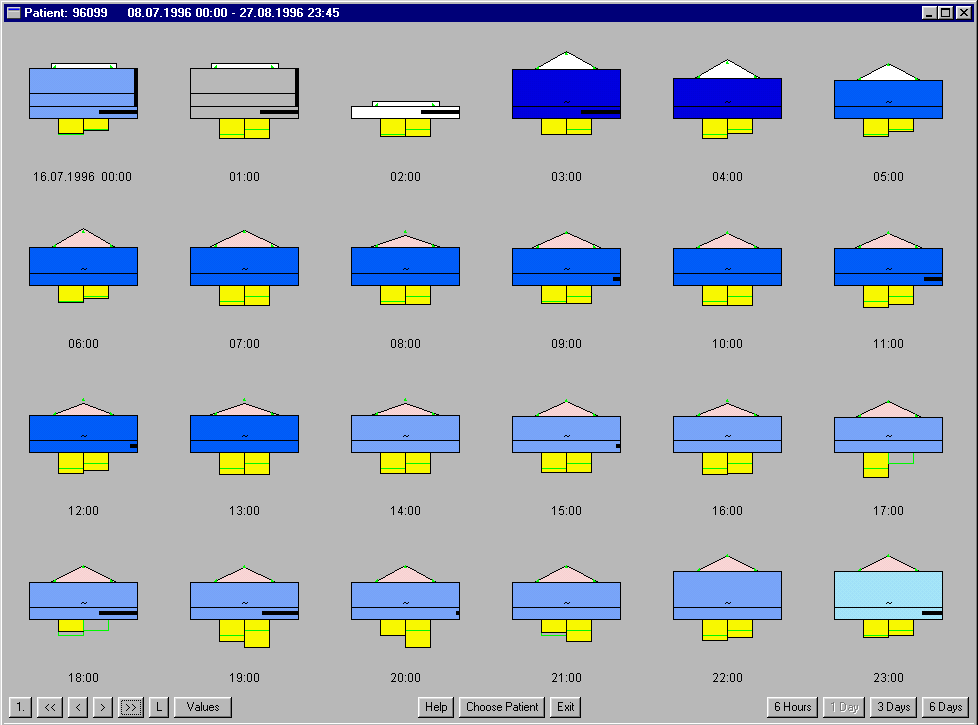
\includegraphics[width=\textwidth]{images/vieVisu.png}
\caption{VIE-VISU is a glyph based visualization for displaying patient vitals~\cite{Horn1998}.}
\label{fig:vieVisu}
\end{figure*}

In some interface implementations, it is conceivable that this connection could be accomplished based on the spatial relationships between prototypes.
For example, placing the left side of one prototype next to the right side of another prototype could trigger a connection between the respective data and property of the primitives.
This visual method of defining connections only works for some spatial relationships. Relationships between color, line weight, or other more abstract spatial properties (area for example) would have to be defined using another interface.

\bodysubsection{Axes and Layout}
\label{axesLayout}

Spatial layout is an important aspect of visualization design.
Administrative data is one of the most common sources of data that influences layout.
For example, in a bar chart, the only actual data on the chart is the vertical height of the bars.
Their horizontal positions come from a sequence, and their vertical position comes from a constant.
The majority of the layout control comes from the step size in the sequence, and the constant mapped to bar width (Figure~\ref{fig:layout}).

\begin{figure*}[t]
\centering
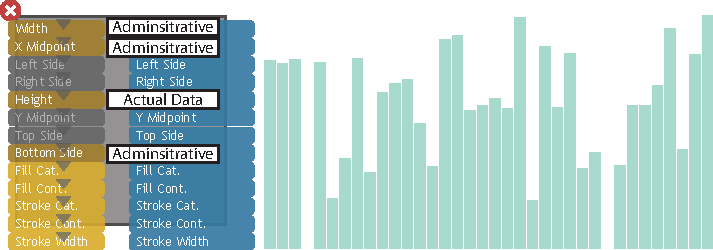
\includegraphics[width=\textwidth]{images/layout.pdf}
\caption{Layout of a bar chart is defined mostly by administrative data.}
\label{fig:layout}
\end{figure*}

The system is limited to layouts that are non-iterative, and do not require spatial information from the layout.
This means that visualizations like tree-maps are not possible, because they subdivide a total space.
This subdivision requires knowing the extents of the total, and iteratively dividing it based on the data.
Word clouds also require iterative layout calculations using information about what is already drawn on the screen.
This feedback loop is not present in the visualization primitives model, as it would require a pipeline approach to achieve.

Axes are not in our current implementation (axes weren't critical for testing creativity), but an axis primitive could provide the labeling necessary.
Its properties would include the label data source, direction, size, etc.
The type of axis could also be driven by a property, switching between a spatial axes or color scale.
The actual labeling could be automatically handled using the extension of Wilkinson's Algorithm by Talbot et al.~\cite{Talbot2010}

Axes are less of an issue for glyphs; the size and position of the objects is entirely relative, there is no axis to compare the spatial dimensions to.
In the case of multiple views (small multiples, trellis displays) that have axes in common, scales exchange information so they can use the same transforms.
This exchange is possible using the output data from each primitive to create connections between the axes present in a visualization.